\subsubsection{Extrapolation assumptions}
\label{sec:HiggsExtrapAss}

%% \textbf{Do we need this introductory text, or will it be discussed in Section 1? In case, it needs to be updated with the corresponding CMS information. --M.D. 2018-11-07} \\

The results presented in this Section are based on the extrapolation to an expected integrated luminosity of 3000~fb$^{-1}$ at $\sqrt{s}$ = 14 TeV of the corresponding ATLAS and CMS Run-2 results. For some of the Higgs decay final states (ATLAS: $WW^*$, $Z\gamma$, $t\bar{t}H$, $\tau\tau$; CMS: $b\bar{b}$) the extrapolation is performed on results obtained with the 2015-2016 36\,$\ifb$ datasets; the remaining final state analyses (ATLAS: $\gamma\gamma$, $ZZ^*$, $b\bar{b}$ and $\mu\mu$) use the results based on the 2015+2016+2017 80\,$\ifb$ data samples. The starting points of the extrapolated results are measurements based on datasets of size $\mathcal{O}(1\%)$ of the expected HL-LHC integrated luminosity. The extrapolations are in this respect very limited with respect to the potential reach of the real HL-LHC analyses, which large statistics will allow to probe corners of the phase space inaccessible at the LHC Run-2.
    
In addition to the increase in integrated luminosity, in most of the studies the extrapolations also account for the increase of signal and background cross-sections from $\sqrt{s}$ = 13 TeV to 14 TeV.  In those cases, the signal yields have been scaled according to the Higgs boson production cross sections values at 13 and 14 TeV, as reported in Ref.~\cite{deFlorian:2016spz}. Similarly, the background yields have been scaled according to the parton luminosity ratio between 13 and 14 TeV, as reported in Ref.~\cite{Heinemeyer:2013tqa}, by taking into account whether the background process is predominantly quark pair or gluon pair initiated.

Object reconstruction efficiencies, resolutions and fake rates are assumed to be similar in the Run-2 and HL-LHC environments, based on the assumption that the planned upgrades of the ATLAS and CMS detectors will compensate for the effects of the increase of instantaneous luminosity and higher pile-up environment at HL-LHC.
%% Experimental uncertainties related to object reconstructions are reduced, neglected or kept untouched depending on the their sources.
For the systematic uncertainties which include experimental, signal and background components, two scenarios have been considered.
The first scenario (S1) assumes the same values as those used in the published Run-2 analyses.
The second scenario (S2) implements a reduction of the systematic uncertainties according to the improvements expected to be reached at the end of HL-LHC program in twenty years from now: the correction factors follow the recommendations from Ref.~\cite{HLHELHCCommonSystematics}.
In certain analyses some of the systematic uncertainties are treated in a specific way, and this is discussed explicitly in each corresponding section.
%
In all analyses, the theory uncertainties for signal and background are generally halved, except where more precise extrapolated values have been provided. Details on the projections of theoretical uncertainties are given in Section~\ref{sec:hl-lhc}. The reduction of the theory uncertainties in gluon-fusion Higgs production is for instance associated to a better understanding of their correlation of their components, leading to their sum in quadrature in scenario S2, instead of the linear sum used in S1 (see Section~\ref{sec:hl-lhc-ggF} for details). The uncertainties related to the PDF are in particular discussed in Section~\ref{sec:2:PDFuncertainties}: these uncertainties are halved in all analyses extrapolation in scenario S2, even though some larger improvements are expected in some cases (e.g. gluon-fusion Higgs production).
%
The uncertainty on the luminosity is set to 1\%.
The uncertainty related to Monte Carlo samples statistics is assumed to be negligible.
%% In the relevant analyses, the spurious signal uncertainty, accounting for backgroundfunctional mismodelling, is also assumed to become negligible.

The extrapolated results are generally limited by systematic uncertainties. It is worth noting that, despite all efforts to design proper projections, the values of the systematic uncertainties of the Run-2 analyses cannot fully account for the HL-LHC conditions and process understanding. The systematic models in current Run-2 analyses are in fact designed for the needs of Run-2, and hence lack flexibility and details needed to account for full-fledged HL-LHC analyses. In this sense, these extrapolated uncertainties are to be considered an approximation. Future analyses will exploit and gain sensitivity from phase space regions that are not accessible yet, or use analysis techniques that reduce the impact of systematic uncertainties.

In the following, all analyses segment the selected events according to the objects produced in association with the Higgs boson decay products and their topology, in order to maximize the sensitivity to the main Higgs production modes ($ggH+b\bar{b}H$, VBF, $VH$ = $qqZH+ggZH+WH$ and top = $t\bar{t}H+tH$)  and to reduce the uncertainties on the respective cross sections. Details on how this segmentation is performed, and on the event selection and categorisation in the various analyses, are found in the Run-2 analysis references quoted in each section.
\subsubsection{$H \to \gamma\gamma$}
\label{sec:Hgammagamma}
%% {\it To be written by: M. Delmastro}

The measurement of the Higgs boson properties in the \Hyy\ channel is performed using the events that contain two isolated photon candidates passing good quality requirements in the precision regions of the detectors. Events are further segmented according to the objects accompanying the diphoton system, in order to maximize the sensitivity to the main Higgs production modes ($\ggF+b\bar{b}H$, VBF, $VH$ = $qqZH+ggZH+WH$ and top = $t\bar{t}H+tH$) and to reduce the uncertainties on the respective cross sections, as well as to the Simplified Template Cross Section (STXS, first introduced in Refs. \cite{deFlorian:2016spz,Badger:2016bpw}) in the merged version of Stage-1.
The Higgs production cross sections are measured for a Higgs boson absolute rapidity $|y_H|$ smaller than 2.5, and with further requirements on the objects campaigning the diphoton system (e.g. jet $p_\mathrm{T}$).
%%
The \Hyy\ signal is extracted by means of a combined signal-plus-background fit of the diphoton invariant mass spectra in the various event categories, where both the continuous background and the signal resonance are parameterized by analytical functions. The shape properties of the signal PDF are obtained by Monte Carlo (MC) simulation, and constrained by performance studies of the photon energy scale and resolution. The background PDF is completely determined by the fit on data, with systematic uncertainties attributed to the specific choice of functional form following the procedure described in Ref. \cite{Aad:2012tfa} or using the discrete profiling method \cite{Dauncey:2014xga}. More details on the analyses methods can be found in most recent measurements in the \Hyy\ channel published by ATLAS \cite{ATLAS:2018uso} and CMS \cite{Sirunyan:2018ouh}. 

The performance of the measurement of the Higgs boson properties in the \Hyy\ channel at HL-LHC is extrapolated from the most recent measurements by ATLAS with 80\,$\mathrm{fb}^{-1}$ \cite{ATLAS:2018uso} and by CMS with 36\,$\mathrm{fb}^{-1}$ \cite{Sirunyan:2018ouh}. The main systematic uncertainties affecting the results are the background modelling uncertainty,
%% QCD scale uncertainties
missing higher order uncertainties
causing event migrations between the bins, photon isolation efficiencies and jet uncertainties.
%% Beside that, the underlying event and parton showering uncertainties as well as the PES and PER play are role.
%
On top of the common assumptions mentioned in Section~\ref{sec:HiggsExtrapAss}, the %ATLAS \Hyy\ 
results of the studies perfromed by ATLAS include a 10\% increase of the background modeling systematic uncertainties, to account for the potentially worst knowledge of the background composition in each analysis category at HL-LHC: this assumption has anyway negligible impact.
%
In the Run-2 analyses, a conservative 100\% uncertainty on the heavy flavour resonant background in top-sensitive categories is applied. Measurements by ATLAS and CMS of the heavy flavour content, or the $b$-jet multiplicity, are expected to better constrain these contributions: for the S2 scenario extrapolation, this uncertainty is therefore halved.

Figure~\ref{fig:Hyy_ATLAS_HLLHC_S2} shows the ratio of the extrapolated \Hyy\ ATLAS measurements of the cross sections times branching fraction of the main Higgs production modes to their respective theoretical SM predictions (left), and uncertainties on these measurements for S1, S2, and stat-only scenarios as extrapolated using the \HZZ\ CMS measurements (right). The reduction of the total uncertainty with respect to the 80\,$\mathrm{fb}^{-1}$ results ranges from a factor of about 2 (3) for the S1 (S2) scenario for the $ggH+b\bar{b}H$, VBF, top cross sections, to a factor of about 5(6) for the $VH$ cross section, that remains dominated by the statistical uncertainty.

\begin{figure}
  \centering
  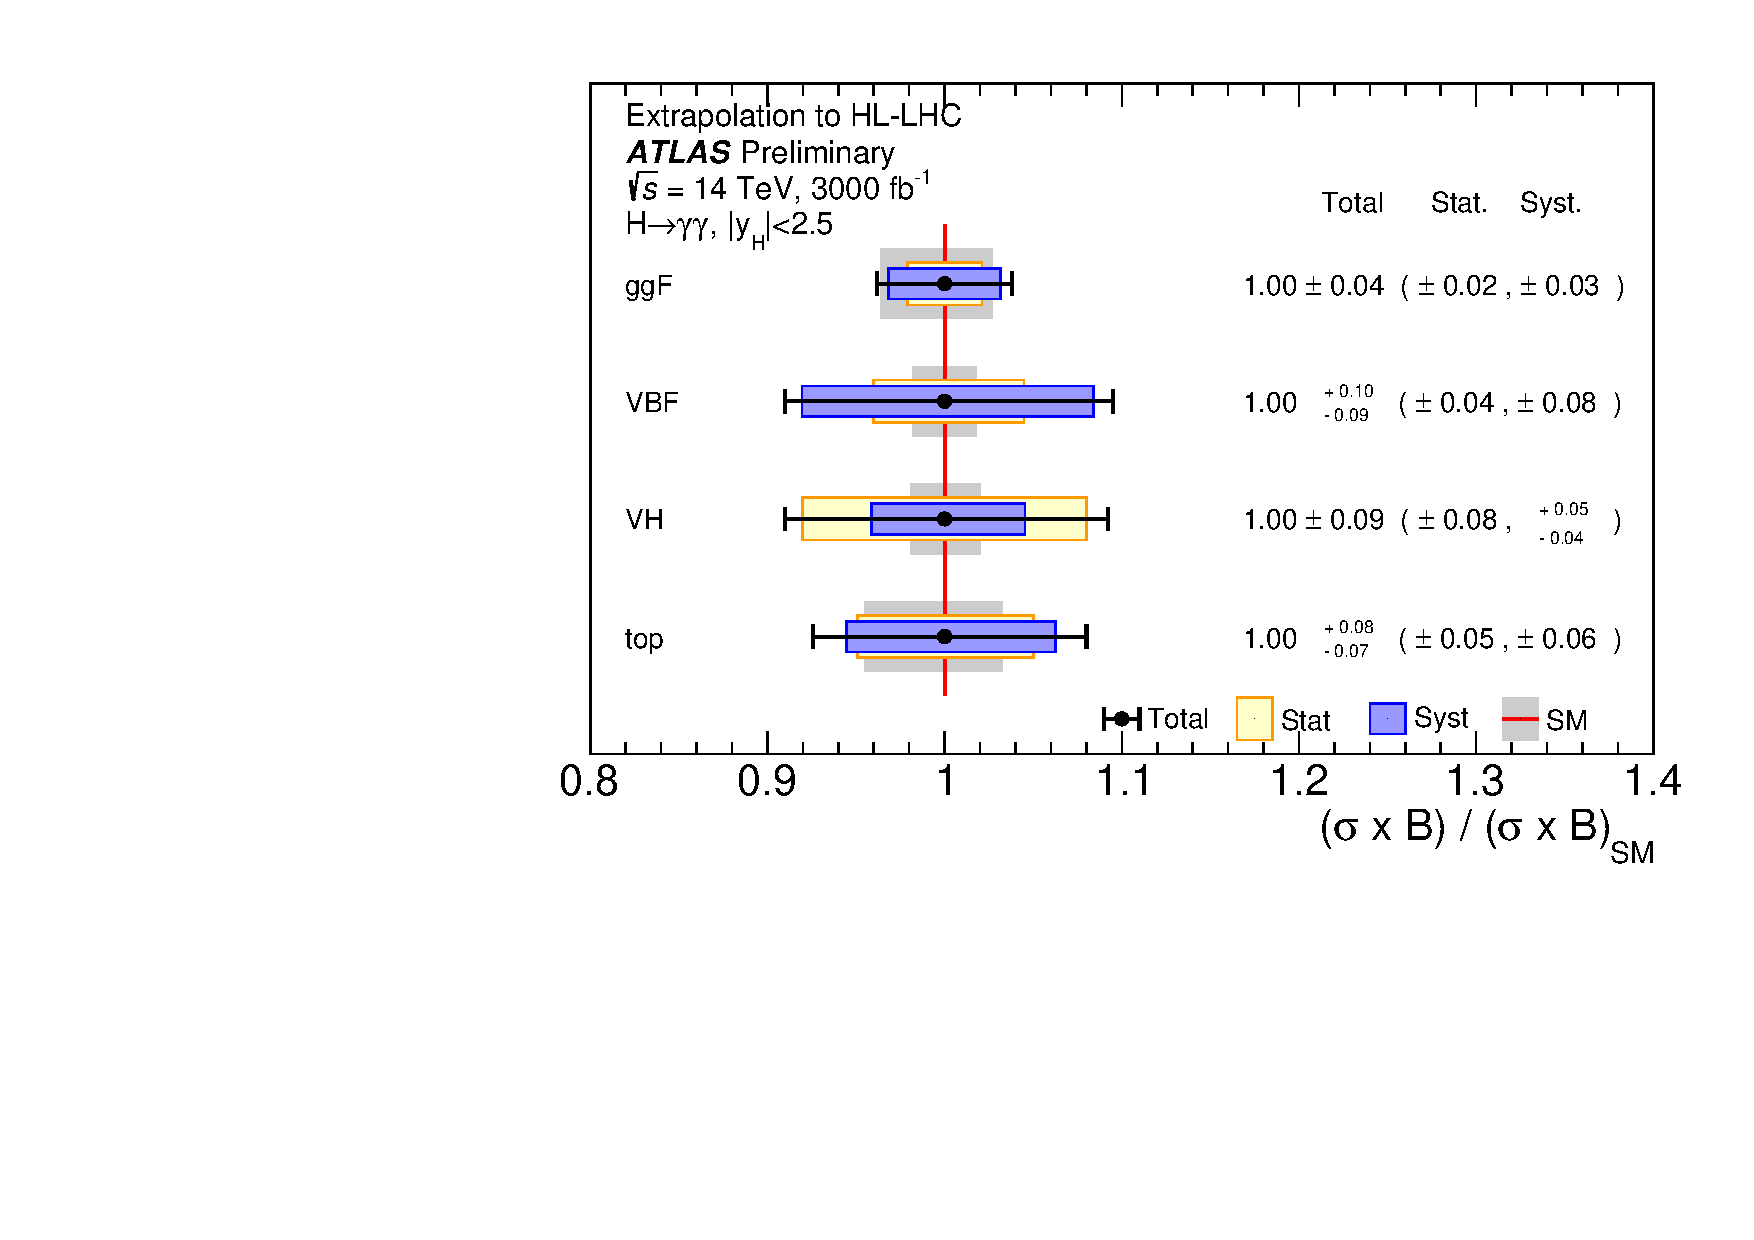
\includegraphics[width=0.56\linewidth]{\main/section2/plots/channels/ATLAS_plot_compareToSM_yy_prodXS}
  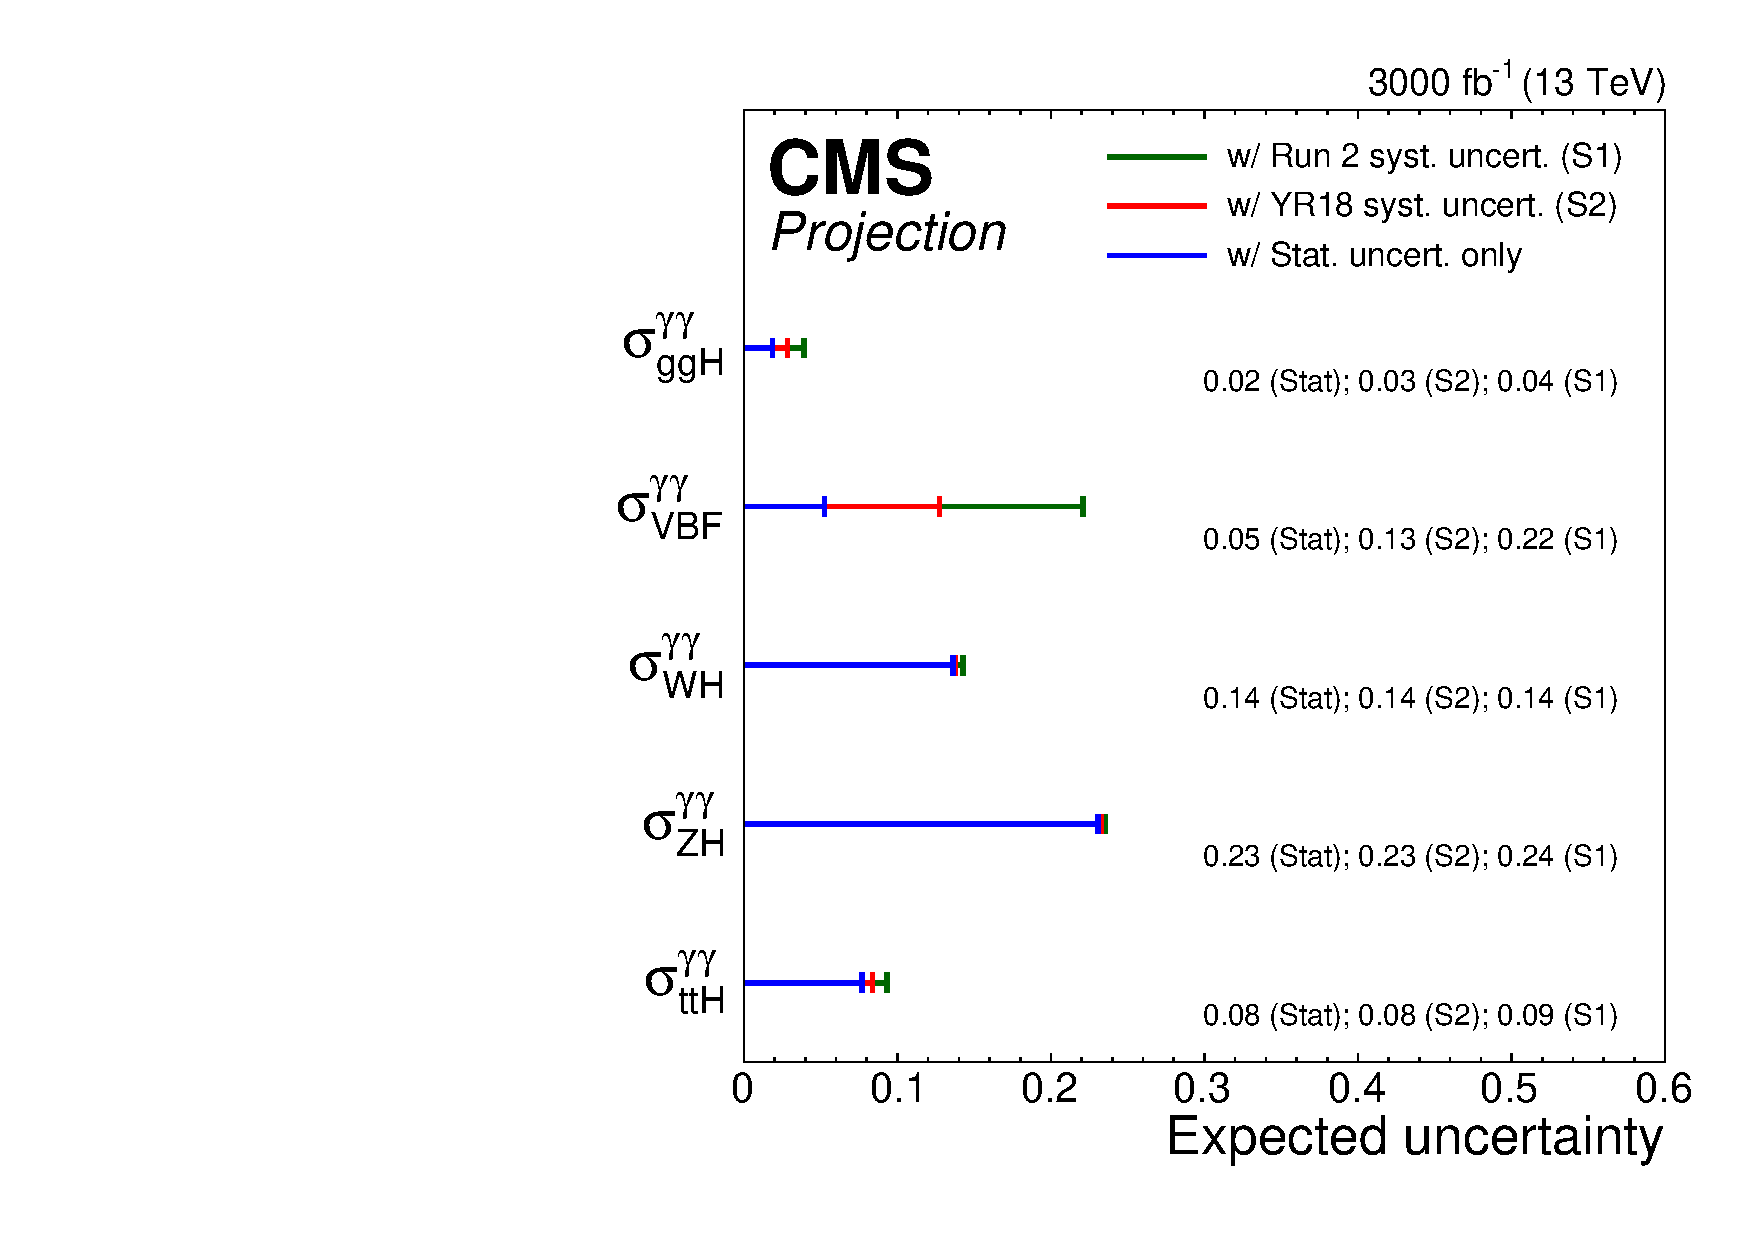
\includegraphics[width=0.42\linewidth]{\main/section2/plots/channels/CMS_summary_A1_5PD_3000_hgg}
  \caption{Cross-section times branching fraction measurements of the main Higgs production modes in the \Hyy\ decay channel, as extrapolated at the HL-LHC. In case of ATLAS results (left) the ratios of cross sections to their respective theoretical SM predictions are shown for scenario S2, while in case of CMS results (right) the uncertainties on these measurements are shown for S1, S2, and Stat-only scenarios..}
  \label{fig:Hyy_ATLAS_HLLHC_S2}
\end{figure}

\subsubsection{$H \to Z\gamma \to \ell\ell\,\gamma$}
%%{\it To be written by: M. Delmastro}

Due to the small branching fraction in the SM, the \HZy\ decay has not yet been observed at the LHC. The experimental observed limits at the $95\%$ confidence level are currently 6.6 times the SM prediction for a Higgs boson mass of 125.09 GeV by ATLAS and 3.9 times the SM prediction for a Higgs boson mass of 125 GeV by CMS, based on the analyses of 36\,$\mathrm{fb}^{-1}$ of $pp$ collision at $\sqrt{s} = 13$ TeV described in Ref. \cite{Aaboud:2017uhw, Sirunyan:2018tbk}.

The analyses select events with an isolated photon candidate passing good quality requirements in the precision regions of the detectors, and a dilepton system with properties compatible with that of the decay of a $Z$ boson. Events are separated according to lepton flavour, the event kinematic properties, and the presence of jets compatible with the VBF production of the Higgs boson, in order to maximize the signal sensitivity. The signal is sought for by means of a combined signal-plus-background fit of the photon-dilepton invariant mass spectra in various event categories, where both the continuous background and the signal resonance are parameterized by analytical functions. The Run-2 analyses are strongly driven by statistical uncertainty, and the main systematic uncertainties are from the bias associated to the background modeling.

The extrapolations to HL-LHC are performed with a simple scaling approach, assuming the same signal and background modeling used in the Run-2 analyses. All experimental and systematic uncertainties are considered to remain the same (S1), except the uncertainty associated to the background modeling, which is taken to be negligible.

The ATLAS expected significance to the SM Higgs boson decaying in $Z\gamma$ is 4.9 $\sigma$ with 3000\,$\mathrm{fb}^{-1}$. Assuming the SM Higgs production cross section and decay branching ratios, the signal strength is expected to be measured with a $\pm0.24$ uncertainty. The cross section times branching ratio for the $pp\rightarrow H \rightarrow Z\gamma$ process is projected to be measured as $1.00\pm0.23$ times the SM prediction. Even at the HL-LHC scenario S1, the analysis sensitivity  to \HZy\ will remain driven by the statistical uncertainty. The dominant source of systematic uncertainty in the extrapolation is that associated to the 
%% QCD scale variations.
missing higher order uncertainties.

\subsubsection{$H \to ZZ^* \to 4\ell$}
%% {\it To be written by: M. Delmastro}

The measurement of the Higgs boson properties in the \HZZ\ channel is performed using the events that contain at least two same-flavour opposite-sign dilepton pairs, chosen from isolated electrons and muons candidates passing good quality requirements in the precision regions of the detectors. Additional constraints on the kinematical properties of the lepton pair associated with the decay of the on-shell $Z$ boson, and on the global topology of the event, helps to improve the signal to background ratio. The four-lepton invariant mass resolution is improved by correcting for the emission of final-state radiation photons by the leptons.
%%
The \HZZ\ signal is extracted from the four-lepton invariant mass spectra in the different event categories, after having evaluated the background components using simulations to constrain their shapes, and data control regions to extrapolate their normalization in the signal regions. Signal to background sensitivity is in general enhanced using the multivariate and/or matrix-element based techniques. More details on the analyses methods can be found in most recent measurements in the \HZZ\ channel published by ATLAS \cite{ATLAS:2018bsg} and CMS \cite{Sirunyan:2017exp}.

The performance of the measurement of the Higgs boson properties in the \HZZ\ at HL-LHC is extrapolated from the most recent measurements by ATLAS with 80\,$\mathrm{fb}^{-1}$ \cite{ATLAS:2018bsg}, and by CMS with 36\,$\mathrm{fb}^{-1}$ \cite{Sirunyan:2017exp}. The dominant systematic uncertainties affecting the extrapolation of the ggH cross section measurement are the lepton reconstruction and identification efficiencies, and pile-up modeling uncertainties. The VBF and VH cross-sections are primarily affected by the uncertainty on the jet energy scale and resolution, and by the
%% QCD scale uncertainties.
missing higher order uncertainties.
These and
%% The theory uncertainties related to QCD scale
the parton shower modeling primarily affects the extrapolated top cross section.

The VBF, VH and especially top measurements in the \HZZ\ decay channel remain largely dominated by statistical uncertainty when extrapolated to 3000\,$\mathrm{fb}^{-1}$ while the $ggH+b\bar{b}H$ cross section is dominated by systematic uncertainties both in scenario S1 and S2.
%
Figure~\ref{fig:HZZ_ATLAS_HLLHC_S2} shows the ratio of the extrapolated \HZZ\ ATLAS measurements of the main Higgs boson production modes to their respective theoretical SM predictions in the scenario S2 (left), and uncertainties on these measurements for S1, S2, and stat-only scenarios as extrapolated using the \HZZ\ CMS measurements (right). The ggF and top \HZZ\ measurements at HL-LHC are expected to reach a level of precision comparable to the projected uncertainty on the corresponding theory predictions.

\begin{figure}
  \centering
  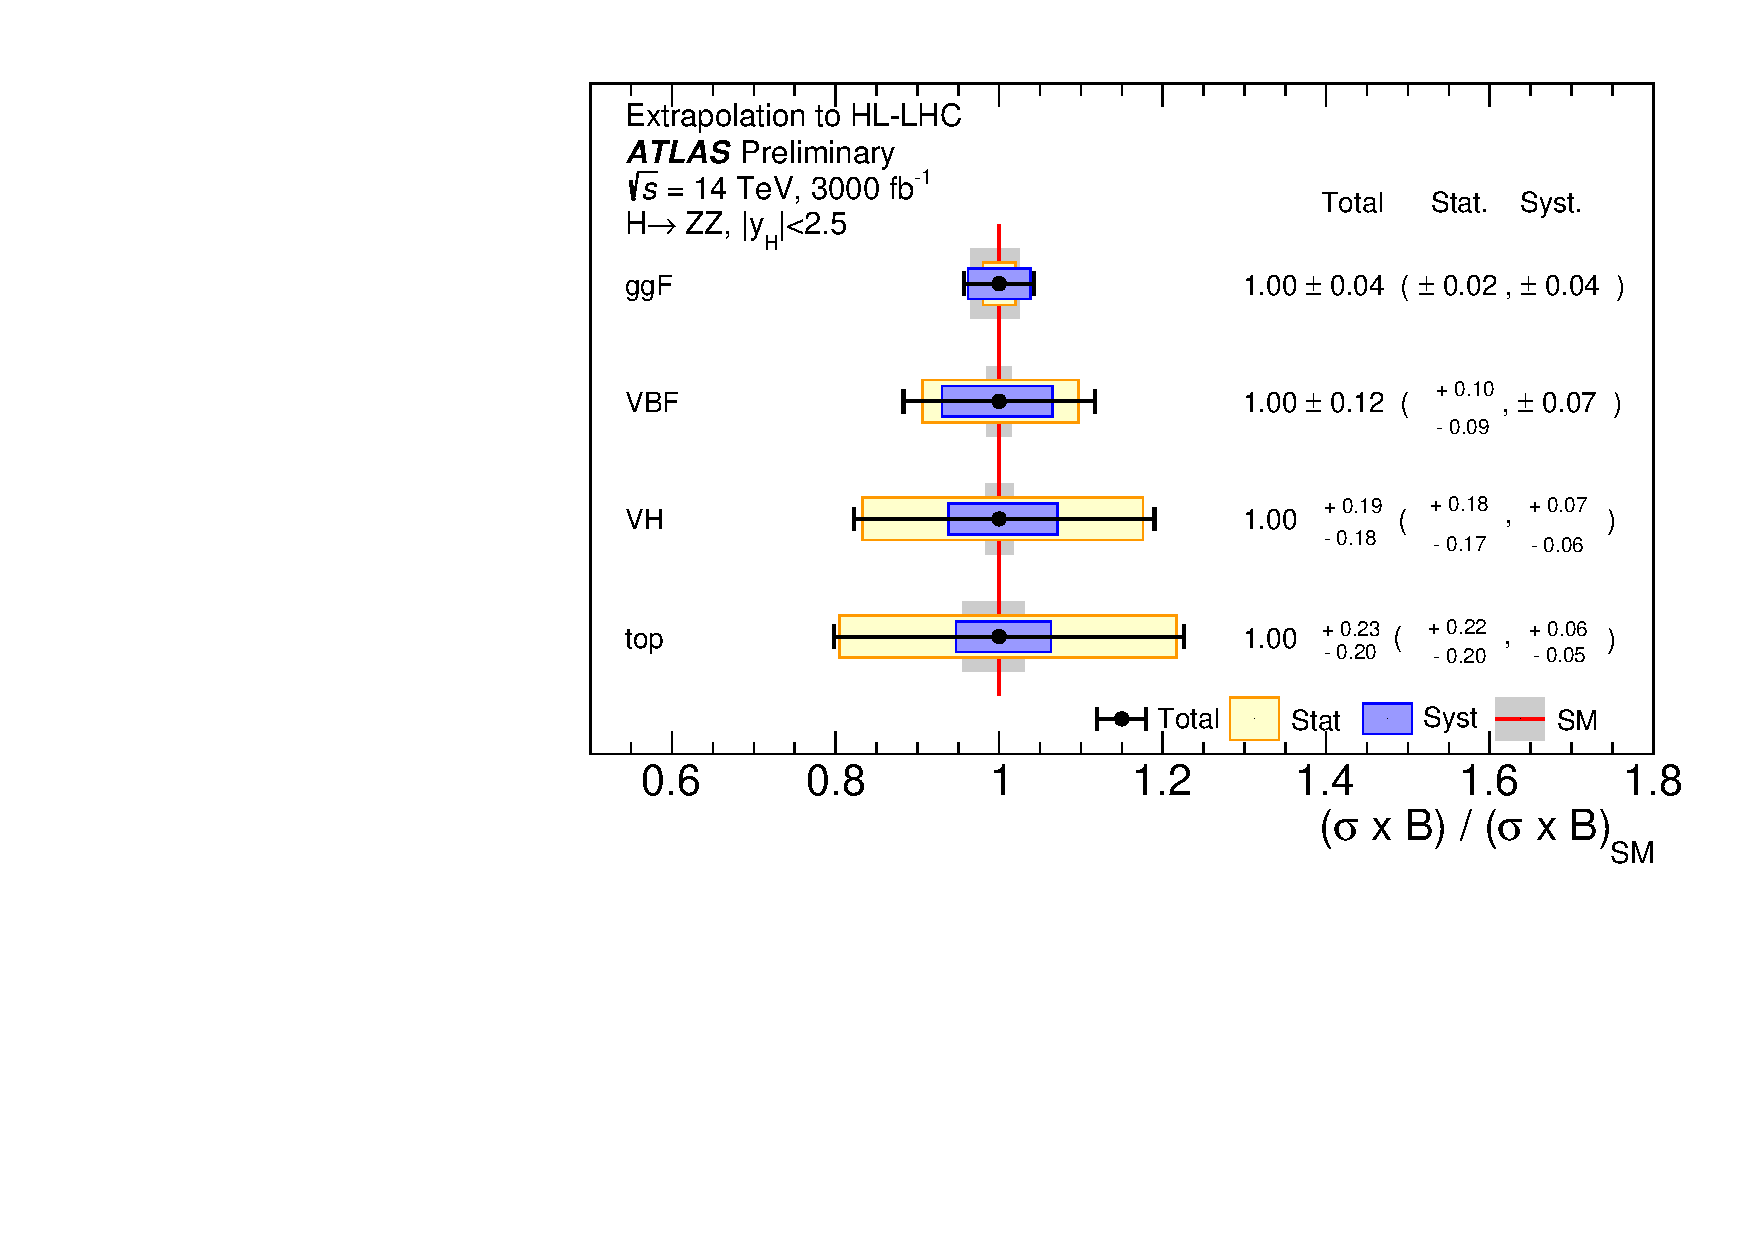
\includegraphics[width=0.56\linewidth]{\main/section2/plots/channels/ATLAS_plot_compareToSM_ZZ_prodXS}
  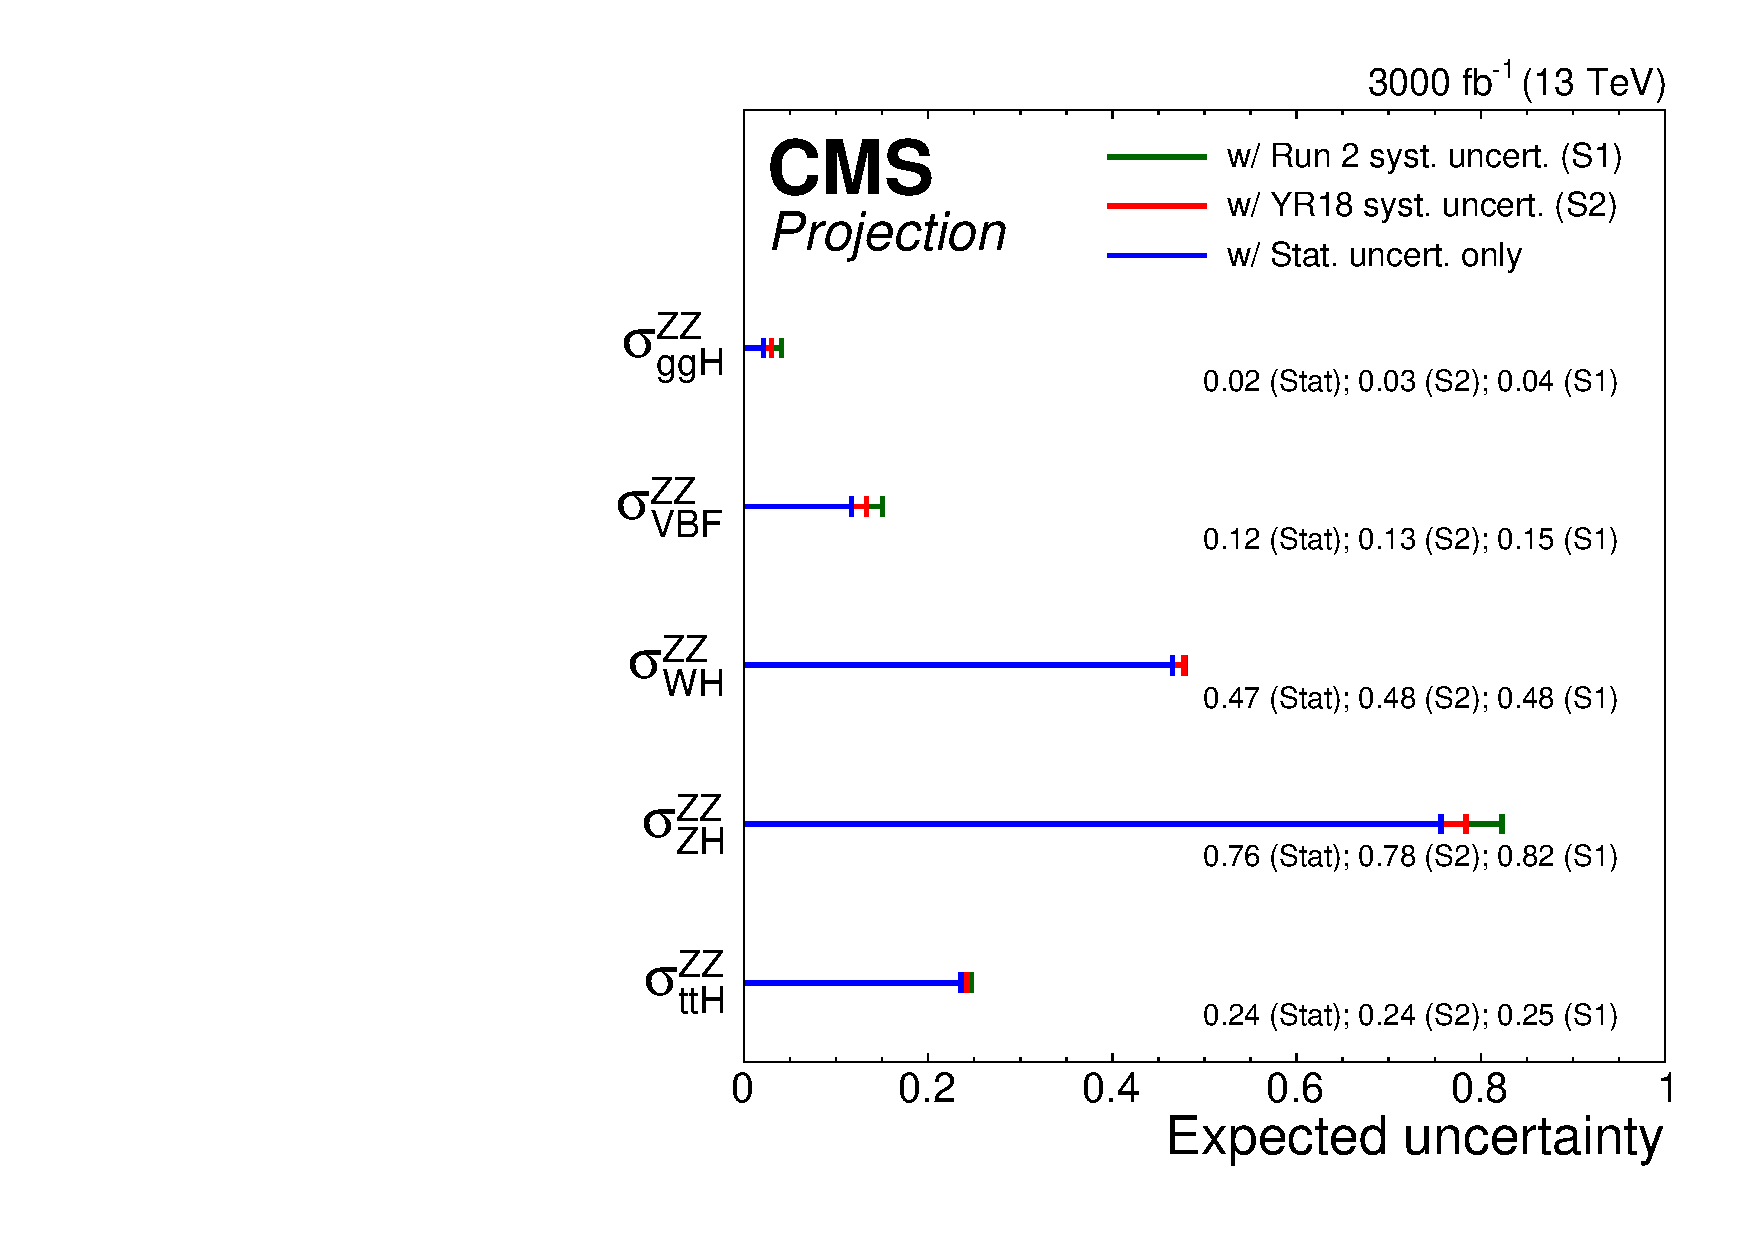
\includegraphics[width=0.42\linewidth]{\main/section2/plots/channels/CMS_summary_A1_5PD_3000_hzz}
  \caption{Cross-section times branching fraction measurements of the main Higgs boson production modes in the \HZZ\ decay channel, as extrapolated at the HL-LHC. In case of ATLAS results (left) the ratios of cross sections to their respective theoretical SM predictions are shown for scenario S2, while in case of CMS results (right) the uncertainties on these measurements are shown for S1, S2, and Stat-only scenarios.}
  \label{fig:HZZ_ATLAS_HLLHC_S2}
\end{figure}

\subsubsection{$H \to WW^* \to \ell\nu\,\ell\nu$}
%% {\it To be written by: M. Delmastro}

The measurement of the Higgs boson properties in the \HWW\ channel is performed using the events that contain two opposite-charged isolated leptons passing good quality requirements in the precision region of the detectors and missing transverse momentum. Additional requirements on the event kinematical properties are applied to reduce the various background components (e.g. requirements on the dilepton invariant mass, transverse mass of the di-lepton + MET system). Events are categorized as a function of the jet multiplicity in order to exploit the different background composition in different categories, and to help extracting the Higgs ggH and VBF production cross sections. The normalizations of the top ($t\bar{t}$ and $W+t$), and $Z\rightarrow\tau\tau$ backgrounds are set using dedicated control regions of the same jet multiplicity as the signal category to which the normalization is transferred. In case of the (non-resonant) $WW$ background, its normalization is either determined using dedicated control regions (ATLAS approach) or by using theoretical prediction with corresponding uncertainty on it (CMS approach). More details on the analyses methods can be found in most recent measurements in the \HWW\ channel published by ATLAS \cite{Aaboud:2018jqu} and CMS \cite{Sirunyan:2018egh}.

The performance of the measurements of Higgs boson properties in the \HWW\ channel at HL-LHC is extrapolated from the most recent measurements in this channel performed by ATLAS with 80\,$\mathrm{fb}^{-1}$ \cite{Aaboud:2018jqu} and by CMS with 36\,$\mathrm{fb}^{-1}$ \cite{Sirunyan:2018egh}. These measurements are completely dominated by systematic uncertainties, and their extrapolation to the S2 scenario shows the expected reduction by a factor two. The measurement of the ggH cross section by branching fraction is dominated by theoretical PDF uncertainty, followed by experimental uncertainties affecting the signal acceptance, including uncertainties on the jet energy scale and flavour composition, and lepton misidentification; the VBF result suffers from similar dominant uncertainties.
%%
Figure~\ref{fig:HWW_ATLAS_HLLHC_S2} shows the ratio of the extrapolated \HWW\ ATLAS measurements of the main Higgs production modes to their respective theoretical SM predictions in scenario S2 (left), and uncertainties on these measurements for S1, S2, and Stat-only scenarios as extrapolated using the \HWW\ CMS measurements (right).

\begin{figure}
  \centering
  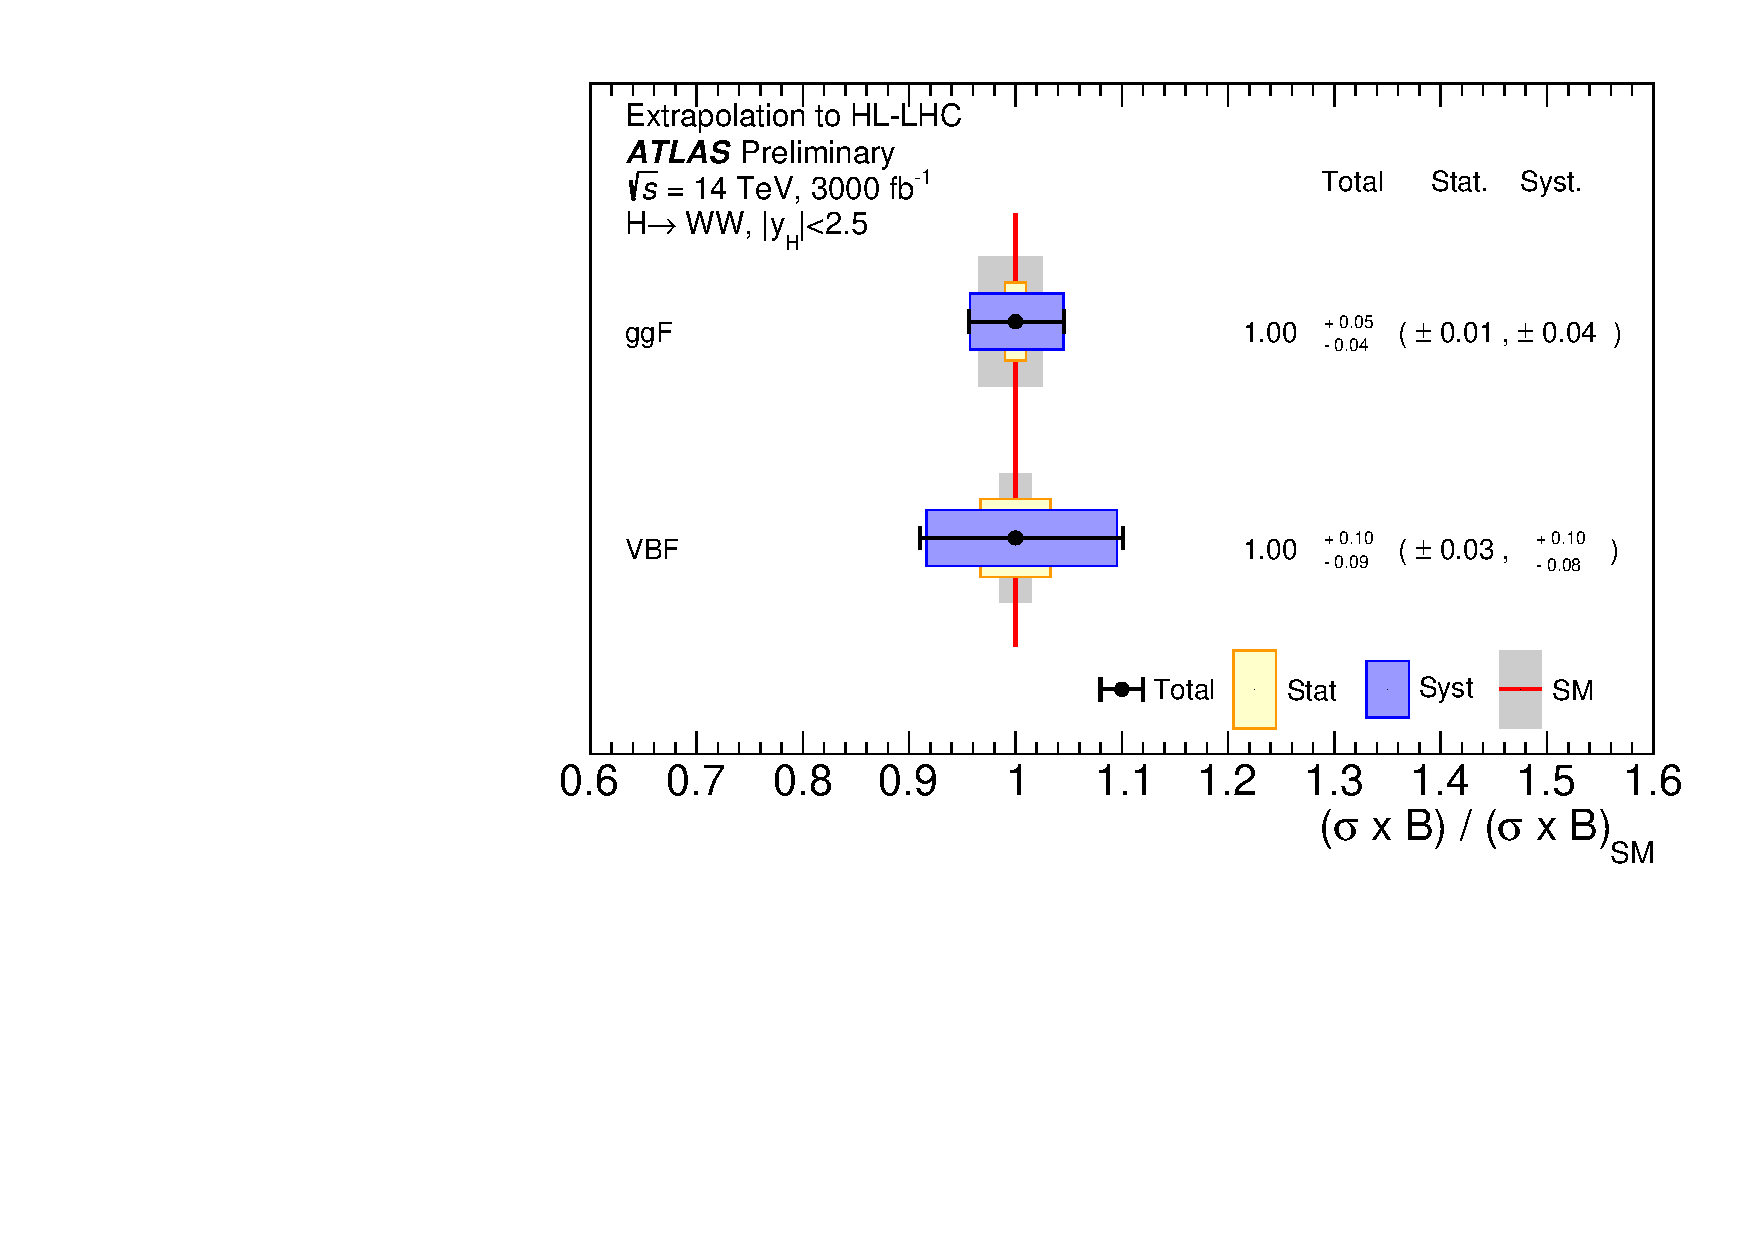
\includegraphics[width=0.56\linewidth]{\main/section2/plots/channels/ATLAS_plot_compareToSM_WW_prodXS}
  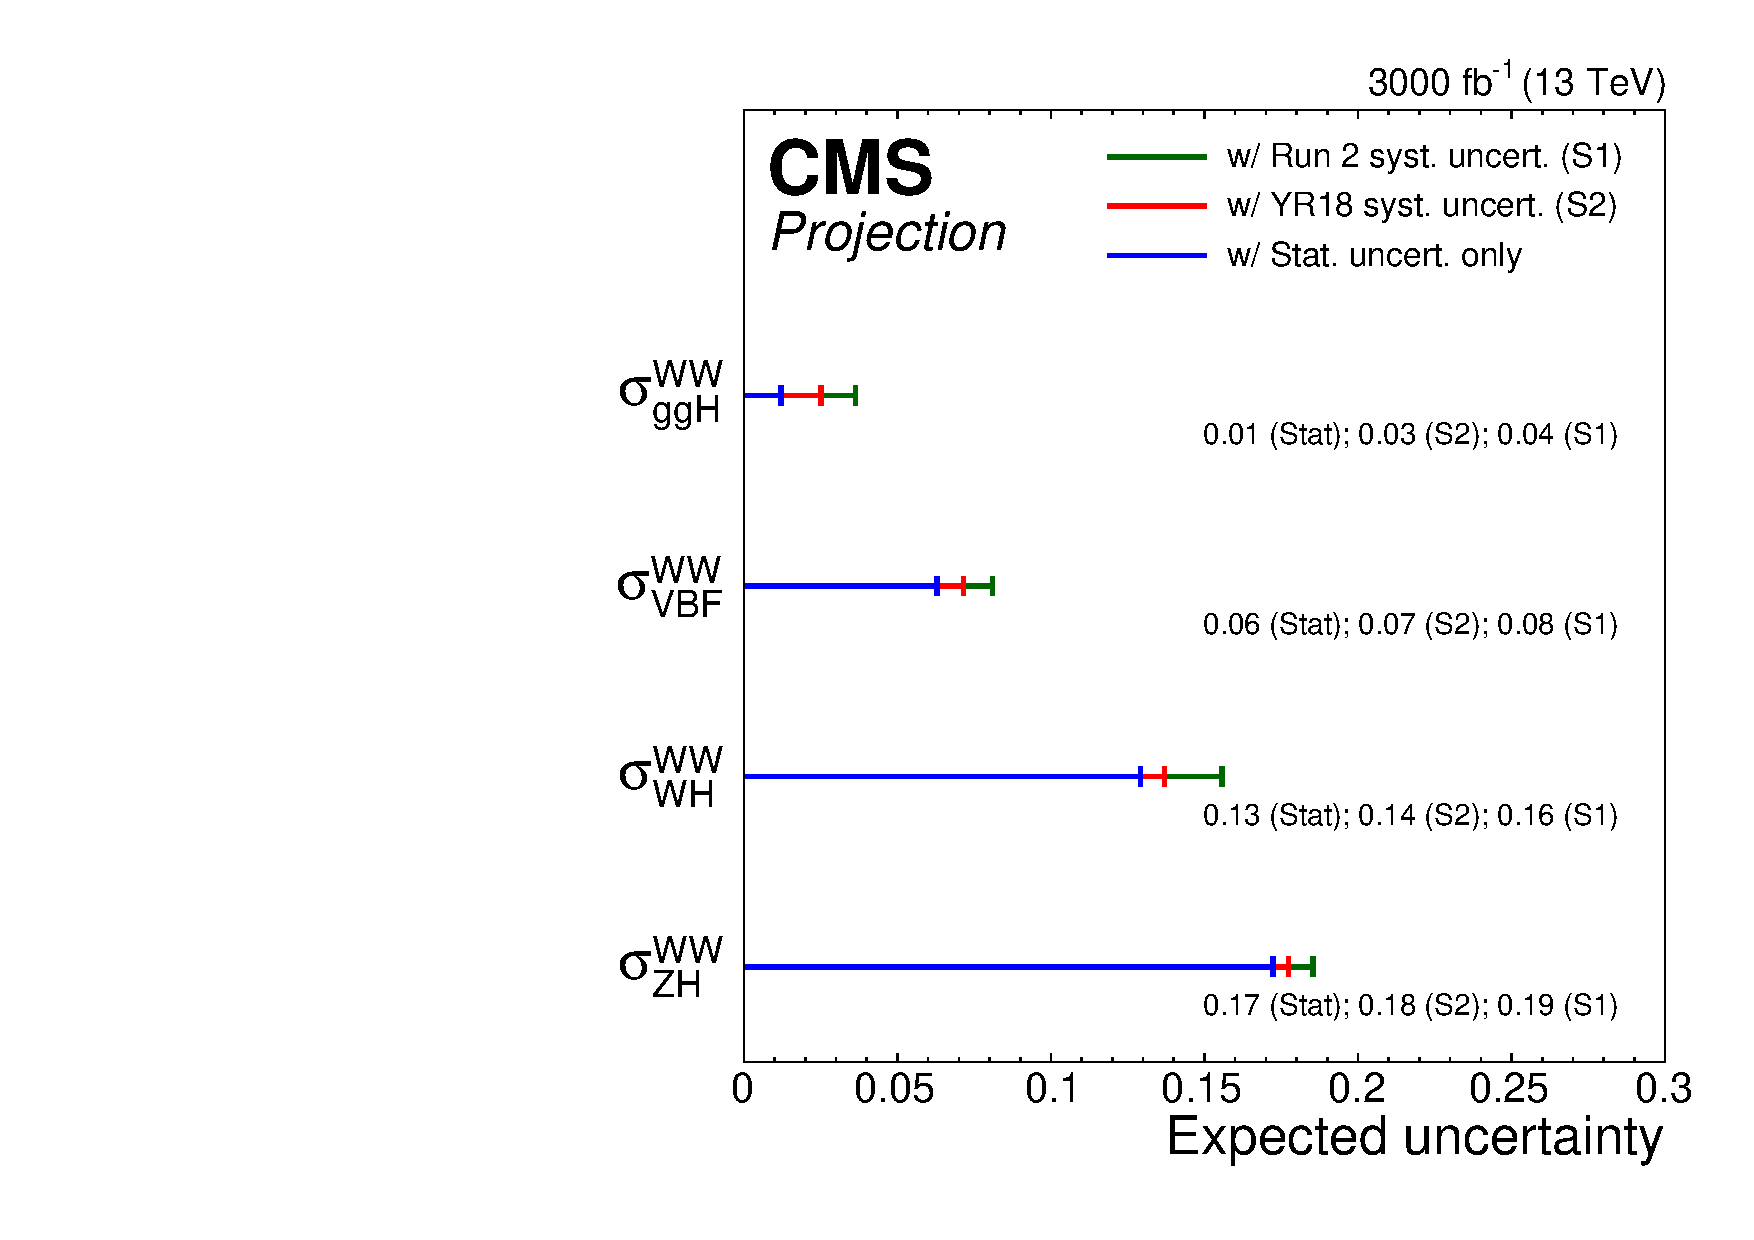
\includegraphics[width=0.42\linewidth]{\main/section2/plots/channels/CMS_summary_A1_5PD_3000_hww}
  \caption{Cross-section times branching fraction measurements of the main Higgs production modes in the \HWW\ decay channel, as extrapolated at the HL-LHC. In case of ATLAS results (left) the ratios of cross sections to their respective theoretical SM predictions are shown for scenario S2, while in case of CMS results (right) the uncertainties on these measurements are shown for S1, S2, and Stat-only scenarios.}
  \label{fig:HWW_ATLAS_HLLHC_S2}
\end{figure}


\subsubsection{$H \to \tau\tau$}
\begin{center}
  \textit{To be written by: P. Francavilla, ?}
\end{center}

%dataset of the extrapolation
The studies presented here are performed based on a previous analysis, in which the ATLAS Collaboration analyzed the 2015/2016 proton-proton collision dataset collected at $\sqrt{s} = 13\,\UTeV$, which corresponds to an integrated luminosity of 36.1\fbinv \cite{}. 
%channels
For the Higgs boson decay products all the leptonic ($\tau_{lep}$) and hadronic ($\tau_{had}$) decays of the $\tau$' s are considered. The analysis is done by splitting events into three categories depending on the three tau final states of the decay products: ($\tau_{lep}$, $\tau_{lep}$), ($\tau_{lep}$, $\tau_{had}$) and ($\tau_{had}$, $\tau_{had}$).

%backgrounds

%results

\subsubsection{$H \to bb$}
{\it To be written by: P. Francavilla, A. de Wit}

\wip{Text currently reflects CMS studies only. Should be updated to reflect ATLAS and CMS studies.
Differences for ATLAS: 
-> the analysis is the observation (78.9 fb-1)
-> tagger is named MVa, and we use a 70\% WP
-> mbb is improved with muon in jet correction and ptReco, + kinematic fit for 2 leptons
-> add the mu for ATLAS
-> Add the results from ATLAS
}

%dataset of the extrapolation
The ATLAS and CMS Collaborations have both reported the observation of the $\text{H}\to\text{bb}$ decay \cite{Aaboud:2018zhk,Sirunyan:2018kst}.
The studies presented here are performed based on a previous analysis, in which 
the CMS Collaboration reported evidence for the $\text{H}\to\text{bb}$ decay in the $\text{VH}$ production mode using the 2016
proton-proton collision dataset collected at $\sqrt{s} = 13\,\UTeV$, which corresponds to an integrated luminosity of 35.9\fbinv \cite{HIG16044}. 
%channels
This analysis makes use of leptonic decays of the vector boson which is produced in association with the Higgs boson. The final states
of the $\vh$ system covered in this analysis always contain two b-jets and either zero, one or two electrons or muons. Both leptons are required to have the same flavour in the two lepton selection.
The b-jets are identified using a combined multivariate (CMVA) tagging algorithm. The inputs include track impact parameter and secondary vertex information from the jet. Three thresholds on the CMVA discriminant are used in the analysis, denoted tight, medium and loose, which have efficiencies for tagging b-jets ranging from $50$--$75\%$ and for light quark or gluon jets from $0.15$--$3\%$.

%backgrounds
Major backgrounds arising from SM production of vector boson plus heavy- or light-flavour jets, in addition to \ttbar production, are 
controlled and constrained for each vector boson decay channel independently via dedicated control regions. Multivariate energy
regression techniques are used to improve the b-jet energy resolution, and a boosted decision tree is used to improve the discrimination 
between signal and background. The distribution of this multivariate discriminator is used as the discriminating
variable in the signal extraction fit. 
%results
The signal strength observed in this analysis is 
$\mu_{\text{VHbb}} = 1.19^{+0.21}_{-0.20}\text{ (stat) }^{+0.34}_{-0.32}\text{ (syst) }$. Here the projected uncertainty
on the signal strength up to 3000\fbinv is reported, assuming $\mu_{\text{VHbb}} = 1$.

Figure \ref{fig:vhbb_projection_intlumi} shows the uncertainty on $\mu_{\text{VHbb}}$ as a function
of integrated luminosity, for scenario S1 (green points), scenario S2 (red points) and a scenario
where all systematic uncertainties are ignored (blue points).
In both scenarios
S1 and S2 systematic uncertainties start to dominate very quickly, thus moving the projected 
uncertainty away from the statistical-only scaling curve.

\begin{figure}[h!]
\begin{center}
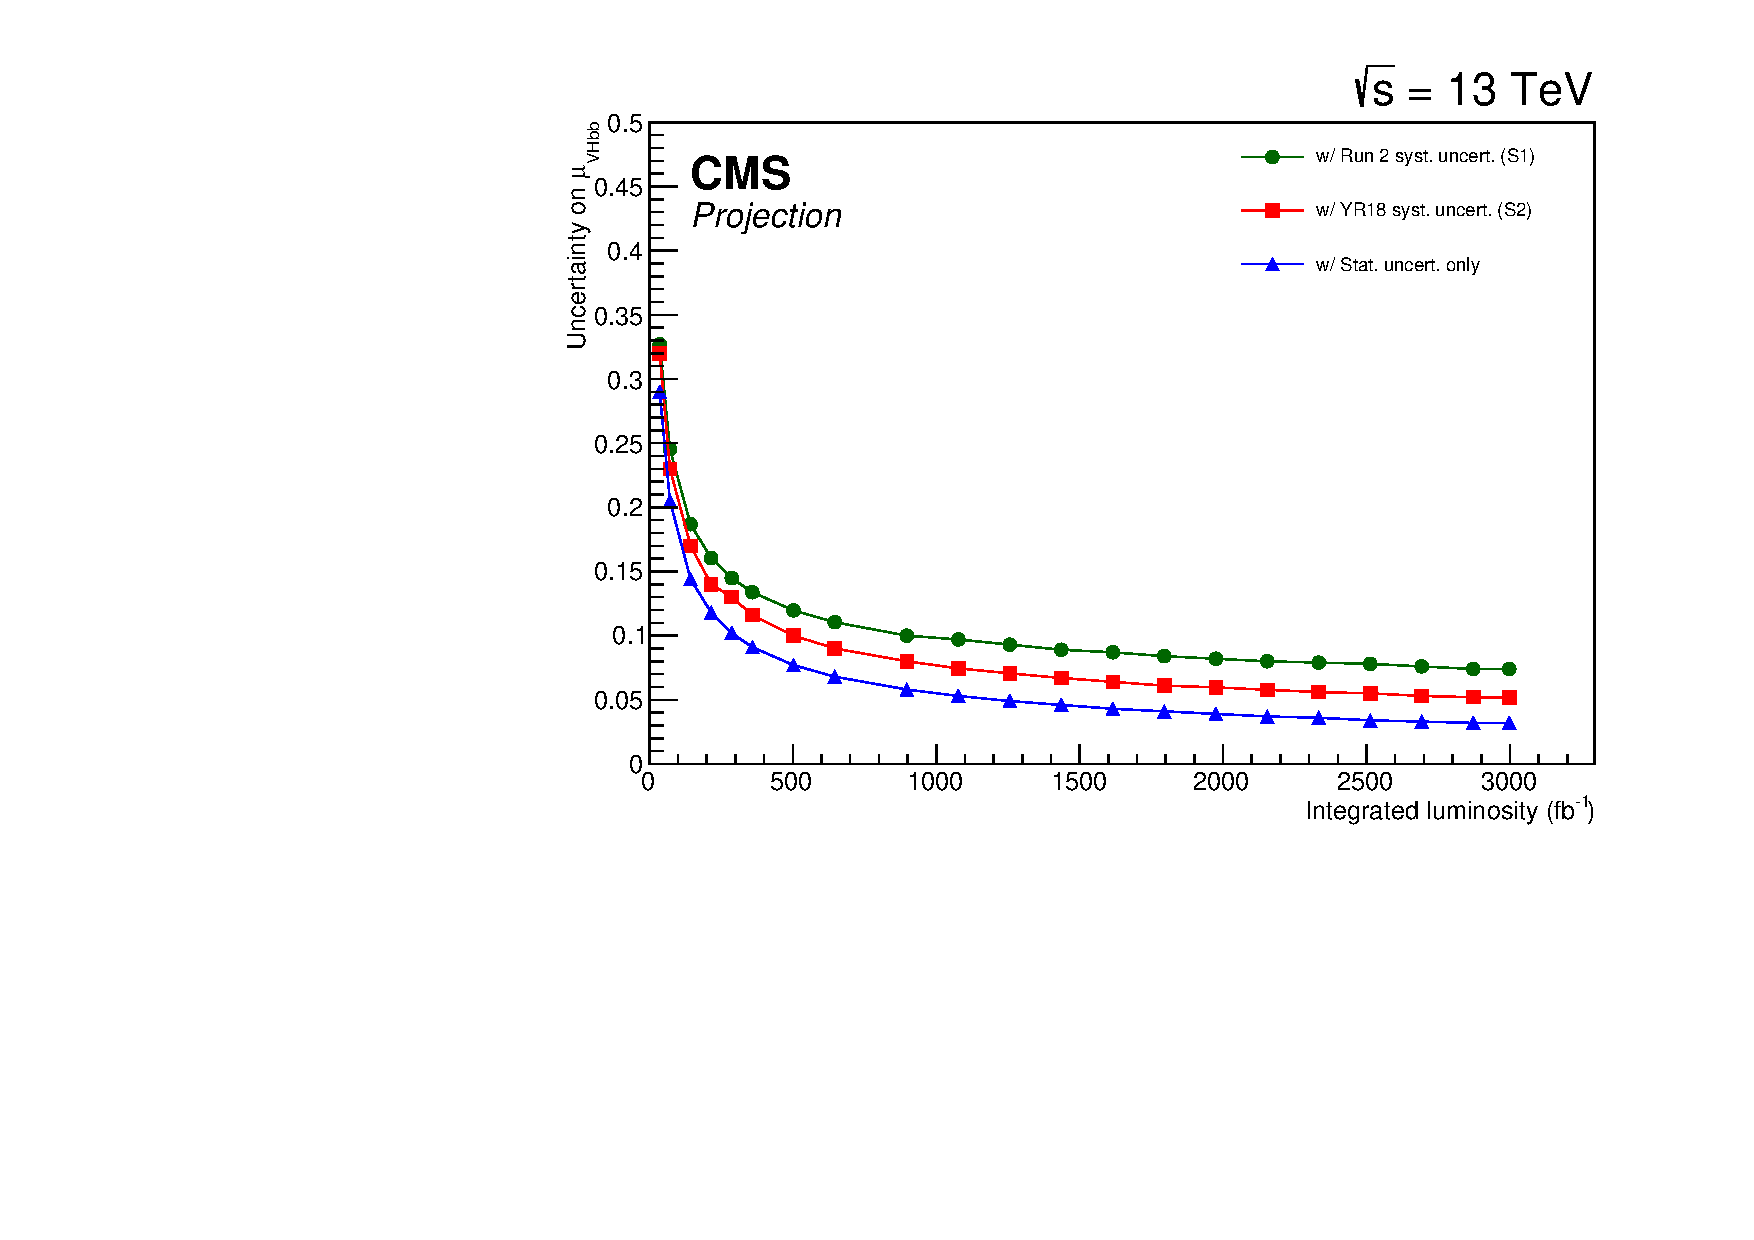
\includegraphics[width=0.75\textwidth]{\main/section2/plots/channels/vhbbprojection_mu_vs_lint.pdf}
\end{center}
\caption{Uncertainty on the signal strength $\mu_{\text{VHbb}}$ as a function of integrated luminosity for S1 (with Run~2 systematic uncertainties~\cite{HIG16044}) and S2 (with YR18 systematic uncertainties).}
\label{fig:vhbb_projection_intlumi}
\end{figure}

Figure \ref{fig:vhbb_proj_bars} shows the per-process and
per-channel signal strength uncertainty, showing results for all three scenarios described above.
The large improvement in the signal strength uncertainty for the 1-lepton channel, which is most sensitive to the WH production
mode, is caused by the integrated luminosity scaling of an uncertainty in the modelling of the $\PW$ boson $\pT$ distribution. This uncertainty dominates this channel
in scenario S1.

\begin{figure}[h!]
\begin{center}
% 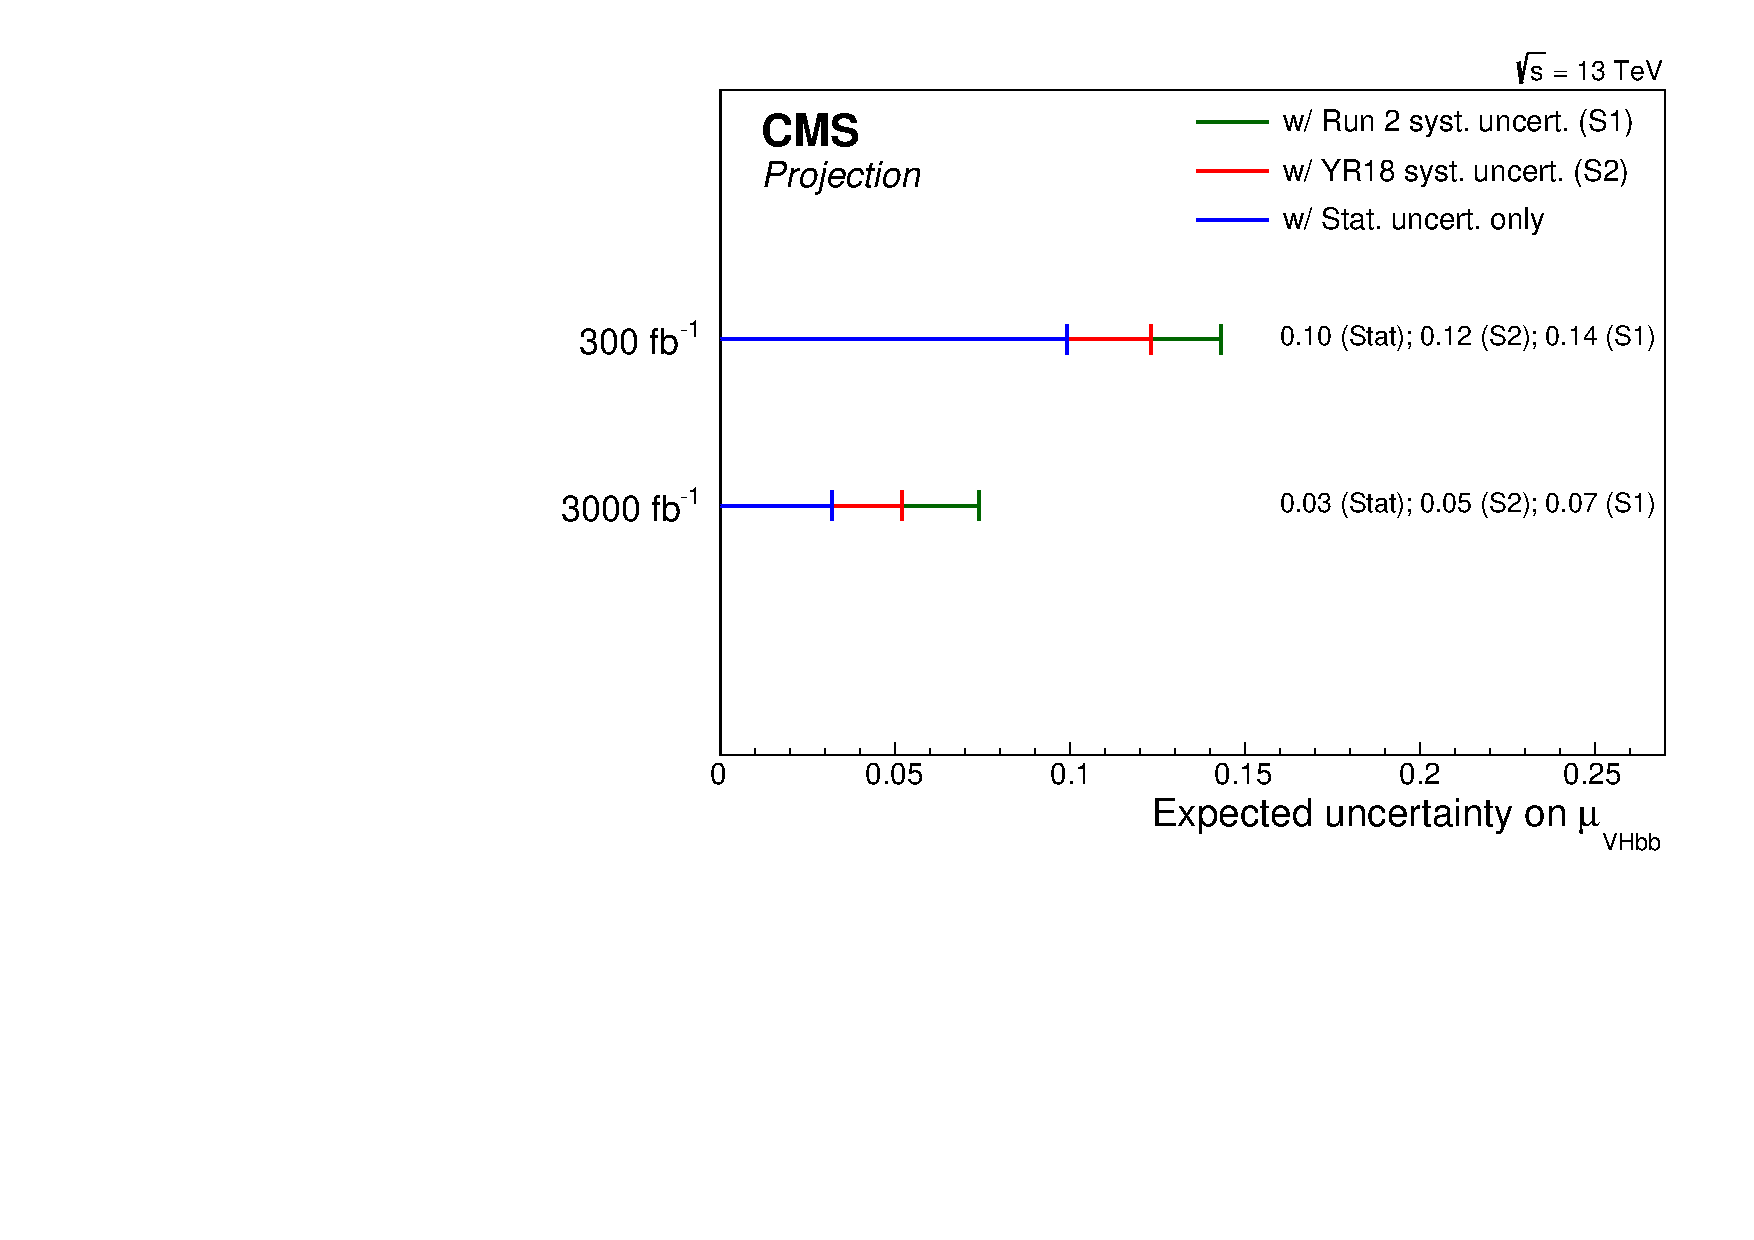
\includegraphics[width=0.48\textwidth]{\main/section2/plots/channels/Uncert300and3000.pdf}
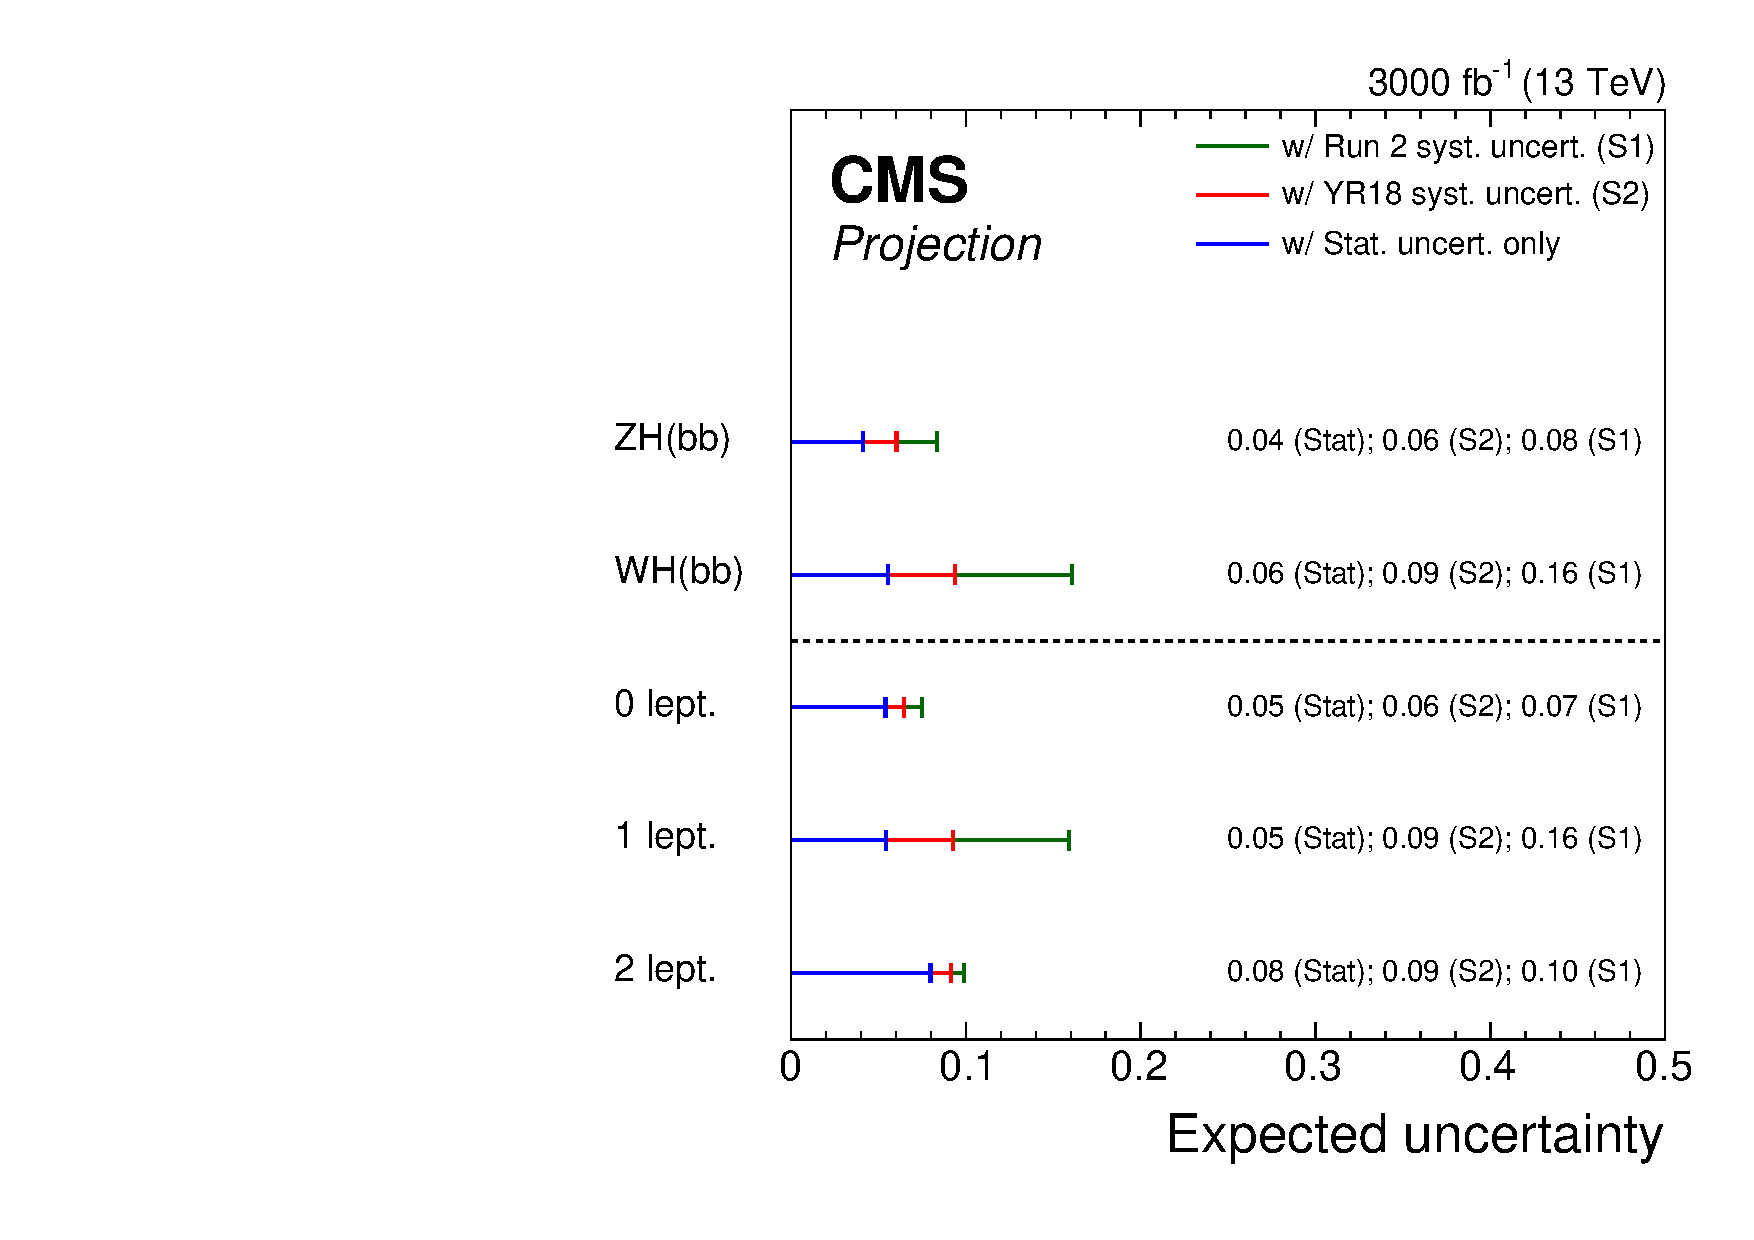
\includegraphics[width=0.6\textwidth]{\main/section2/plots/channels/ccc_3000fb_all.pdf}
\end{center}
\caption{Uncertainties in the per-process and per-channel signal strengths. Values are given for the S1 (with Run~2 systematic uncertainties~\cite{HIG16044}) and S2 (with YR18 systematic uncertainties) scenarios, as well as a scenario in which all systematic uncertainties are removed.}
\label{fig:vhbb_proj_bars}
\end{figure}

The contributions of different sources of uncertainty in scenarios S1 and S2 are shown in Table~\ref{tab:vhbb_uncertbreakdown}.
Both in scenario S1 and S2 the largest component of the systematic uncertainty is theoretical. Moving from S1 to S2 the total signal theoretical uncertainty reduces to half its size. This is expected as in scenario S2 the input uncertainties
are scaled down to half the current size. In the case of the background theory, where the input uncertainties are also scaled to half their original
size when going from scenario S1 to scenario S2, the total uncertainty due to this component is not halved. This is because at 3000 \fbinv
some of the theoretical uncertainties on the backgrounds can be constrained in the fit. The same is true for the experimental uncertainties, which
in some cases are already moderately constrained in the current analysis.

Looking in more detail at the dominant signal theoretical uncertainties, the largest component in the uncertainty arises from the uncertainty in the gluon-induced $\zh$ ($\ggZH$) production cross section due to QCD scale variations.
The $\ggZH$ process contributes a small fraction of the total $\zh$ process. Despite this, the uncertainty in the production cross section for this process due to QCD scale variations 
becomes dominant because it is very large: 25\% for the ggZH process, compared to approximately 4\% for the ZH process \cite{deFlorian:2016spz}.
The next most important uncertainties are category-acceptance uncertainties in the dominant Z+bb and W+bb backgrounds due to QCD scale variations, as well as the uncertainty in the ZH and WH production
cross section due to QCD scale variations. In scenario S2 these four most important uncertainties contribute 1.6\%, 1.5\%, 1.3\% and 1.2\% (absolute) to
the total uncertainty of 5.1\%, respectively. To improve the precision of the measurement it is therefore important to improve these theoretical uncertainties.

\begin{table}[th!]
\begin{center}
{
\caption{Contributions of particular groups of uncertainties in S1 (with Run~2 systematic uncertainties~\cite{HIG16044}) and S2 (with YR18 systematic uncertainties). The total uncertainty is decomposed into four components: signal theory, background theory, experimental and statistical. The signal theory uncertainty is further split into inclusive and acceptance parts, and the contributions of the b-tagging and JES/JER uncertainties to the experimental component are also given.}
\label{tab:vhbb_uncertbreakdown}
\begin{tabular}{l c c}
 & S1 & S2\\
Total uncertainty   & 0.073  & 0.051 \\
\hline
Signal theory uncertainty& 0.054 & 0.026\\
\quad Inclusive & 0.046 &0.022\\
\quad Acceptance & 0.027 &0.013\\
Background theory uncertainty & 0.028 & 0.023\\
Experimental uncertainty & 0.026 & 0.022 \\
\quad b-tagging & 0.022  & 0.020 \\
\quad JES and JER & 0.007  & 0.006 \\
Statistical uncertainty & 0.032 & 0.032\\
\end{tabular}
} % end footnotesize
\end{center}
\end{table}

In the future, and at the HL-LHC in particular, the b-tagging efficiency may change. The conditions could worsen the efficiency, but
at the same time new detectors and new techniques could also lead to an improvement in the b-tagging efficiency. 
The effect of changes in b-tagging efficiency on the overall signal strength uncertainty is evaluated. Changes in the b-tagging
efficiency are emulated by scaling the rates of processes with a single b-tag by the change in b-tagging efficiency, and scaling the 
rates of processes with two b-tags by the change in b-tagging efficiency squared. The modifications are applied only to the efficiency to select genuine b-jets; the mistagging rates for light quark and gluon jets remain unchanged.

Figure \ref{fig:vhbb_btageff} shows the results of the projection assuming various reductions and improvements in the b-tagging efficiency relative to the performance of the three CMVA working points used in the analysis.
A 10\% improvement in the b-tagging efficiency leads to a relative improvement in the signal strength uncertainty of up to 6\%. The improvements on the signal strength precision are limited because the uncertainty is dominated by theoretical sources. When neglecting inclusive signal theory uncertainties this improvement becomes up to 8\%. \wip{Results at $300\fbinv$ will be removed from the plot.}


\begin{figure}[h!]
\begin{center}
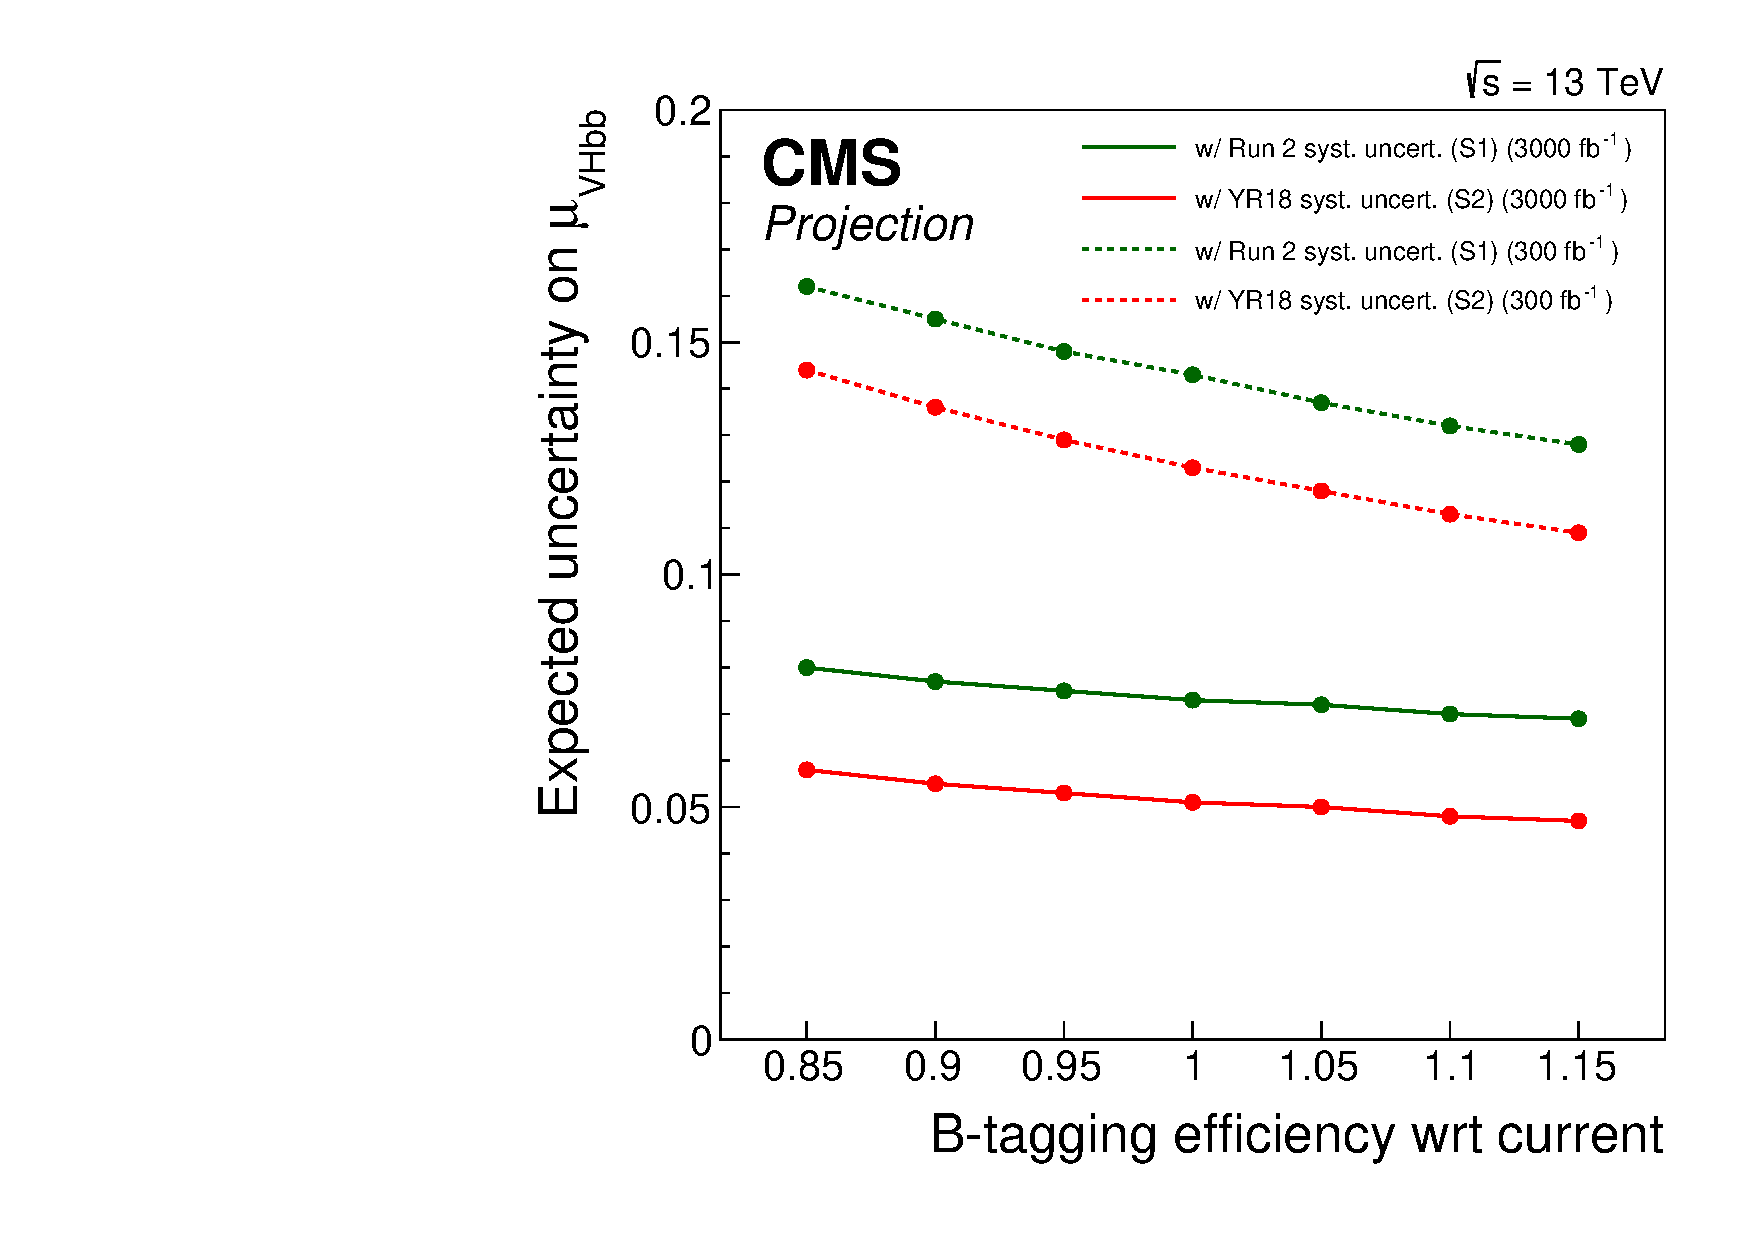
\includegraphics[width=0.5\textwidth]{\main/section2/plots/channels/BTagEff_Fig.pdf}
\end{center}
\caption{Effect of varying the b-tagging efficiency on the uncertainty in the signal strength measurement when considering all systematic uncertainties.}
\label{fig:vhbb_btageff}
\end{figure}

\subsubsection{$H \to \mu\mu$}
{\it To be written by: P. Francavilla, ?}
